\documentclass[tikz,border=8pt]{standalone}
% Shared look for every TikZ diagram. Load with \input{../../tools/tikz-style.tex}
\usepackage[T1]{fontenc}
\usepackage{lmodern}
\renewcommand{\sfdefault}{lmr}  % diagrams use the same serif as the text
\usetikzlibrary{arrows.meta, positioning, shapes.geometric, calc, fit, backgrounds}
\definecolor{cblue}{HTML}{4C78A8}
\definecolor{corange}{HTML}{F58518}
\definecolor{cgreen}{HTML}{54A24B}
\definecolor{cred}{HTML}{E45756}
\definecolor{cpurple}{HTML}{B279A2}
\definecolor{cgrey}{HTML}{6B6B6B}
\tikzset{
  every picture/.style={font=\sffamily, line width=1.2pt},
  box/.style={draw=#1, fill=#1!12, rounded corners=4pt, align=center, inner sep=7pt, minimum height=1.1cm},
  box/.default=cgrey,
  arrow/.style={-{Stealth[length=3mm]}, draw=cgrey, line width=1.4pt},
  title/.style={font=\sffamily\bfseries\Large},
  note/.style={font=\sffamily\small, text=cgrey, align=center},
}
\AtBeginDocument{\hyphenpenalty=10000 \exhyphenpenalty=10000}

\begin{document}
\begin{tikzpicture}[node distance=0.5cm]
  \node[box, text width=2.2cm] (x) {flower\\ $x = (1, x_1, x_2)$};
  \node[box, right=1.2cm of x, yshift=1.1cm, text width=2.6cm, fill=cblue!15] (z1) {$z_1 = w^{(1)} \cdot x$};
  \node[box, right=1.2cm of x, text width=2.6cm, fill=corange!15] (z2) {$z_2 = w^{(2)} \cdot x$};
  \node[box, right=1.2cm of x, yshift=-1.1cm, text width=2.6cm, fill=cgreen!15] (z3) {$z_3 = w^{(3)} \cdot x$};
  \foreach \n in {z1, z2, z3} \draw[arrow] (x.east) -- (\n.west);
  \node[box, right=1.0cm of z2, text width=2.4cm, minimum height=3.2cm] (sm) {\textbf{softmax}\\[4pt] $\hat{y}_k = \dfrac{e^{z_k}}{\sum_j e^{z_j}}$};
  \foreach \n in {z1, z2, z3} \draw[arrow] (\n.east) -- (sm.west |- \n.east);
  \node[box, right=1.0cm of sm, text width=2.5cm] (p) {three probabilities\\ adding up to 1};
  \node[box, right=0.8cm of p, text width=2.1cm] (c) {predict the largest};
  \draw[arrow] (sm) -- (p); \draw[arrow] (p) -- (c);
  \node[note, below=0.45cm of z3, text width=3cm] {one weight vector per class};
\end{tikzpicture}
\end{document}
